\chapter[Prenatal endocrine disrupting chemical exposure \& child IQ]{Prenatal endocrine disrupting chemical exposure \& child IQ: {\LARGE Accounting for uncertainty in pattern identification in a two-stage health analysis}}\label{sec:ch4}
\vspace{-3em}

\begin{center}
Elizabeth A. Gibson,\textsuperscript{1} 
Robbie M. Parks,\textsuperscript{1}
Pam Factor-Litvak,\textsuperscript{2} 
Jeff Goldsmith,\textsuperscript{3} 
John Paisley,\textsuperscript{4} 
Julie B. Herbstman,\textsuperscript{1} 
Marianthi-Anna Kioumourtzoglou\textsuperscript{1} \\ 

\textbf{Affiliations:} \\ 1. Department of Environmental Health Sciences, Columbia University; \\ 
2. Department of Epidemiology, Columbia University; \\ 
3. Department of Biostatistics, Columbia University; \\ 
4. Department of Electrical Engineering, Columbia University. 
\end{center}

\clearpage

%% main text

\section{Introduction}
The prevalence of neurodevelopmental disorders in the U.S. has increased over previous decades \citep{boyle2011trends}. Even a small downward shift may have a substantial population impact \citep{gore2015edc}. In a large population, a five-point reduction in IQ results in a doubling in the absolute number of individuals with IQ scores consistent with intellectual disabilities (IQ $<$ 70) \citep{braun2017early}, which has further downstream consequences for reduced societal productivity and economic loss \citep{bellanger2015neurobehavioral}. To inform the design of strategies promoting neurological health, we must identify modifiable risk factors, such as environmental contributors, including EDCs endocrine disrupting chemicals (EDCs) \citep{sathyanarayana2008phthalates, gore2015edc}. EDCs, such as phenols and phthalates, specifically, appear as plasticizers, preservatives, and additives in a wide variety of personal care products and food packaging, making exposure ubiquitous \citep{philippat2015exposure, schettler2006human, lorber2015exposure, koniecki2011phthalates}. 

Phenols and phthalates are not chemically bound to products, causing human exposure through inhalation, absorption, and ingestion \citep{vandenberg2007human}, and both cross the placenta during pregnancy \citep{schonfelder2002parent, mose2007phthalate}. Mounting evidence connects EDC exposures, such as phthalates \citep{van2020phthalate, nidens2020prenatal, kim2018association, doherty2017prenatal, kim2011prenatal}, triclosan \citep{jackson2018identifying, guo2020early}, parabens \citep{freire2020association}, and bisphenol A (BPA) \citep{jiang2020prenatal, lin2017prenatal}, during the critical \textit{in utero} period with adverse child cognitive development in childhood. Within the Columbia Center for Children’s Environmental Health's (CCCEH) Mothers and Newborns birth cohort, we have previously reported associations between prenatal exposure to individual phthalates and child cognitive development \citep{factor2014persistent, whyatt2012maternal}. Because associations between single EDCs and cognition do not encompass collective exposure to multiple chemicals simultaneously, interest in EDCs as an environmental mixture continues to increase \citep{braun2016can, taylor16}. Research has broadened to include joint and interactive effects among chemicals \citep{hu2021prenatal}, EDC mixture exposure profiles \citep{kalloo2021chemical}, and the overall effect of the EDC mixture \citep{tanner2020early}.

Here, we investigate a mixture of 17 phenols and phthalate metabolites measured in spot urine samples collected during the third trimester of pregnancy. To assess exposure to all EDCs simultaneously and to identify patterns within the mixture, we consider the high dimensionality of the exposure matrix and the complex correlation structures across the chemicals \citep{taylor16}. We propose a two-stage Bayesian model for estimating health effects of patterns of environmental exposures. In the first stage, we fit a non-parametric non-negative matrix factorization (\bnmfc) that performs pattern recognition within an environmental mixture (Cite: \bnmfc); subsequently, we propagate the uncertainty from the first stage in a hierarchical regression model to estimate the association between exposure patterns and the health outcome. The primary goal of this research is to describe relationships between \bnmfc-identified patterns of \textit{in utero} EDC exposure (while properly incorporating our confidence in these patterns) and child cognition at seven years of age.

\section{Methods}

\subsection{Study Population}
For this study, we included a subset of mother-child dyads enrolled in the CCCEH Mothers and Newborns longitudinal birth cohort. This cohort study was initiated to evaluate the effects of prenatal exposure to air pollutants on birth outcomes and cognitive and behavioral development in children. A total of 727 African American and Dominican women were recruited from two prenatal clinics in Northern Manhattan between 1998 and 2006. Enrollment, exclusion criteria, and a description of the cohort have been described previously \citep{perera03}.

We included mothers in the current study if phthalate metabolite and phenol concentrations were measured in their spot urine samples collected during pregnancy (n = 343). We included all mothers with chemical measurements in the pattern identification step (see Section ~\ref{sec.patterns}). Children were selected for participation in the health analysis if their mothers were included in the pattern identification and if they completed the Wechsler Intelligence Scale for Children, 4th edition (WISC-IV) at age 7 years (n = 311). We saw no significant differences between these subsets and the overall Mothers and Newborns cohort in WISC full scale IQ or covariates (see Supplemental Table~ref{table:suptable1}). Participating mothers provided written informed consent for themselves and their child, children provided their assent to participate beginning at age 7, and Columbia University Medical Center's Institutional Review Board approved the study procedures.

\subsubsection{Phthalate \& phenol measurements}
We collected spot urine samples during the third trimester of pregnancy. Eight environmental phenols (Benzophenone-3 (BP-3), triclosan, 2,4-dichlorophenol (24-DCP), 2,5- dichlorophenol (25-DCP), methyl paraben (M-PB), propyl paraben (P-PB), butyl paraben (B-PB), and bisphenol A (BPA)) and nine phthalate metabolites (Mono-2-ethylhexyl (MEHP), mono-2-ethyl-5-carboxypentyl (MECPP), mono-2-ethyl-5-hydroxyhexyl (MEHHP), mono-2-ethyl-5-oxohexyl (MEOHP), mono-benzyl (MBZP), mono-3-carboxypropyl (MCPP), mono-n-butyl (MBP), mono-isobutyl (MIBP) and mono-ethyl (MEP)) were measured at the U.S. Centers for Disease Control and Prevention (CDC) as described previously \citep{ye2005automated, calafat2008exposure, silva2004urinary}. The limits of detection (LODs) ranged from 0.2 to 2.3 ng/ml urine for phenols and 0.2 to 2.3 ng/ml urine for phthalates. Concentrations of phenols and phthalate metabolites were specific gravity-adjusted to account for urinary dilution \citep{hauser2004temporal}. These markers are non-persistent, and repeated measures have show inconsistency over time in other samples \citep{fisher2015bisphenol}. However, previous research in the Mothers and Newborns cohort showed moderate reliability over a short time span, approximating continuous exposure. Intra-class correlation coefficients were 0.77 for MBZP, 0.65 for MnBP, 0.60 for MIBP, and between 0.27 and 0.42 for the di(2-ethylhexyl) phthalate (DEHP) metabolites \citep{whyatt2012maternal, factor2014persistent}.

\subsubsection{Child intelligence measurement}
The Wechsler Intelligence Scale for Children, 4th edition (WISC-IV) was administered to children at age seven \citep{wechsler2003wechsler}. The WISC-IV full scale intelligence quotient (IQ) represents a child's general intellectual performance across four indices: verbal comprehension, perceptual reasoning, working memory, and processing speed. The WISC-IV has been validated among both English- and Spanish-speaking populations and has been shown to be sensitive to low-dose exposure of certain individual phthalates and phenols \citep{factor2014persistent, guo2020prenatal}.

\subsubsection{Model covariates}
\label{sec:cov}
Extensive data were collected using medical records and questionnaires administered during pregnancy. Potential confounders included maternal age, intelligence, and education (less than high school vs. at least high school or equivalent), marital status (ever married vs. never married), and material hardship (any reported vs. none reported). Strong predictors of the outcome included alcohol use during pregnancy (any wine, beer, or liquor vs. none) and quality of the care-taking environment (measured at child age three). The quality of the home environment was measured by the Home Observation for Measurement of the Environment (HOME) scale \citep{caldwellhome}. Maternal intelligence was assessed by the Test of Non-Verbal Intelligence, third edition, a language-free measure of general intelligence \citep{brown1990test}. We scaled continuous covariates (maternal age, IQ, and HOME score) to mean zero and standard deviation one. Seven percent of eligible children were excluded (n=22 of N=311) due to missing covariate data. We examined the data for patterns between variables with missing values and others using a Kruskal-Wallis test to compare with continuous variables and a chi-squared test for discrete variables. We confirmed that missingness did not relate to any other data in the dataset, i.e., variables were missing completely at random (MCAR).

\subsection{Statistical analysis}
We examined distributional plots and descriptive statistics for all variables. We assigned phthalate metabolite and phenol concentrations below the limit of detection (LOD) the value of $LOD/\sqrt{2}$ \citep{hornung1990estimation}. We scaled all concentrations to standard deviation equal to 1 prior to the pattern identification step. Analyses were conducted using R version 4.0.4 and Stan version 2.26 \citep{rrr, gelman2015stan}. 

\subsubsection{Pattern identification}
\label{sec.patterns}
\bnmf is a pattern recognition tool which reduces the dimensionality of a chemical mixture, expressing individual exposure in terms of their underlying patterns. \bnmfc-identified individual scores and chemical loadings are similar to frequentist non-negative matrix factorization (NMF) in their interpretation. Non-negativity puts the results on the same range as the original chemical concentrations and provides solutions interpretable on an additive scale with a parts-based representation \citep{holtzman2018machine, lee1999learning}. \bnmf is distinct from traditional NMF in two important ways. First, the Bayesian framework allows for uncertainty in estimation. This is expressed as a distribution around individual scores and chemical loadings on patterns. In this work, we incorporated the distributions around individual point estimates as hierarchical exposures in the health model (see Section~\ref{sec.health}), which included our confidence in the pattern recognition step in the 95\% credible intervals around $\beta$ coefficients. \bnmfc's non-parametric prior on the number of patterns in a mixture also distinguishes it from other NMF methods, which require an \textit{a priori} specification or \textit{post-hoc} selection of pattern number. \bnmf helps to remove the researcher from specification and selection of pattern number, estimating it from the data. Here, we used individual scores on \bnmfc-identified patterns across 17 phthalates and phenols measured in pregnant women from a previous analysis (Cite: \bnmfc).

For a matrix $X =\lbrace x_{i j}\rbrace $ of $i = 1:N$ individuals and $j = 1:P$ chemicals, \bnmf identifies matrices $W$ and $H$ and the vector $\mathbf{a}$ arising from the following data generating process,
\begin{equation}
\label{nmf}
X_{i j} \sim \operatorname{Poisson}\left(\sum^K_{k=1} W_{i k} \mathbf{a}_k H_{k j}\right)
\end{equation}

Where $K$ is the number of patterns determined by the model. $W$, $H$, and $\mathbf{a}$ all have Gamma priors; the Gamma distribution is over non-negative real numbers, so this enforces non-negativity on the solution. The vector $\mathbf{a}$ has a sparse Gamma prior to optimally shrink the number of patterns. We obtained individual scores from the posterior distribution, ${W\operatorname{diag}(\mathbf{a}) \sim \operatorname{Gamma}(\alpha_W, \beta_W)} \times
\operatorname{Gamma}(\alpha_\mathbf{a}, \beta_\mathbf{a})$. The expectation of this distribution, $\mathbb{E}[\widehat{W}\operatorname{diag}(\widehat{\mathbf{a}})]$, represents individuals' exposure concentrations on the $K$ identified patterns. We also obtained chemicals loadings from the posterior distribution, $H \sim \operatorname{Gamma}(\alpha_H, \beta_H)$. The expectation, $\mathbb{E}[\widehat{H}]$, defines each pattern's unique mixture of chemical loadings.

To standardize values from \bnmfc, we normalized chemical loadings over patterns (i.e., divided each loading by the sum of all loadings on a pattern) and multiplied individual scores by their corresponding normalization constant. This put individual scores on different patterns on the same scale. We further transformed patterns to have standard deviation equal to one across individual scores to enable interpretation of the coefficient size in the subsequent regression model as corresponding to a one standard deviation increase in the exposure pattern.

\subsubsection{Health models}
\label{sec.health}
\paragraph{Traditional models.} We conducted multivariable linear regression analyses to evaluate the relationships between prenatal EDC exposure patterns and continuous full scale IQ scores. We refer to these models as `traditional' throughout this work because environmental health and epidemiological research has traditionally worked within a frequentist framework. We ran pattern-specific models for $\mathbb{E}[\widehat{W}_1\widehat{\mathbf{a}}_1]$ and $\mathbb{E}[\widehat{W}_2\widehat{\mathbf{a}}_2]$, adjusting for covariates, because identified patterns were not correlated ($r$ = -0.07). We place `hats' on these quantities to emphasize that they were estimated by \bnmf in the first stage of our analysis. Final regression models included covariates that were \textit{a priori} defined as potential confounders based on previous literature and a directed acyclic graph, or that were strong predictors of full scale IQ (see Section~\ref{sec:cov}) \citep{pearl2009causality, hernan2010causal}. We used penalized splines to investigate deviations from linearity and determined that linear models fit the data well. Because there is a large body of evidence indicating sex-specific associations between endocrine disrupting chemicals and health outcomes, we included sex as an effect modifier in all models and present sex-specific results.

We identified influential outliers using Studentized residuals, which scale each residual by its corresponding standard deviation, and Cook's distance, which measures the effect of deleting a given observation on the remaining data \citep{kleinbaum2013applied}. Two observations with values $>$ 5 standard deviations from  the phthalate + BPA pattern mean were identified and removed for the main analysis.

\paragraph{Bayesian hierarchical models.} Because our traditional regression models did not account for the inherit uncertainty in the first stage of this analysis, we next fit Bayesian health models. This allowed us to incorporate the distributional information from \bnmf in the regressions. \bnmf generated individual scores from the product of two Gamma distributions, $\widehat{W}$ and $\widehat{\mathbf{a}}$, and we used these distributions to build a hierarchical likelihood as follows,
\begin{equation}
\begin{aligned}
Z_i & \sim \operatorname{Gamma}(\widehat{\alpha}_{W i}, \widehat{\beta}_{W i}) 
    \times \operatorname{Gamma}(\widehat{\alpha}_{\mathbf{a} i},
    \widehat{\beta}_{\mathbf{a} i})  \\
Y_i & = \beta_0 + \beta_Z Z_i + \beta_{S} S_i 
+ \beta_{Z \cdot S} \left(Z_i S_i\right) 
+ \mathbf{X}_{i}^T\boldsymbol{\beta}_\mathbf{X} + \varepsilon_i \\
\end{aligned}
\end{equation}

For $i = 1 ... N$, $Z_i$ is the individual pattern score drawn from the distribution estimated by \bnmfc, with scale and rate parameters $\widehat{\alpha}_{W i}$ and $\widehat{\beta}_{W i}$ for the distribution over $\widehat{W}_i$ and $\widehat{\alpha}_{\mathbf{a} i}$ and $\widehat{\beta}_{\mathbf{a} i}$ for the distribution over $\widehat{\mathbf{a}}_i$. The outcome $Y_i$ is continuous full-scale IQ; $\beta_0$ is the intercept;  $S_i$ is child's sex; $Z_i S_i$ is the interaction term between individual pattern score and sex; and $\mathbf{X}_{i}$ is a vector of additional covariates. The regression coefficients \(\beta_Z\), \(\beta_S\), \(\beta_{Z \cdot S}\), and \(\beta_\mathbf{X}\) relate their subscript to the outcome, and $\varepsilon_i$ is residual error.

We left improper, non-informative priors on $\beta$'s and $\varepsilon$, putting equal weight on all real numbers for $\beta$ coefficients, \(\mathbb R \), and over all non-negative real numbers, \(\mathbb R_{\geq 0}^+\), for the intercept ($\beta_0$) and the standard deviation of the error term ($\varepsilon \sim \mathcal{N}(0,\sigma^2)$). These priors are improper in that they did not integrate to one (though the posterior does) and non-informative in that they were dominated by the data and played a minimal role in the posterior distribution. This made the results more comparable to those from our traditional regression.

\subsubsection{Sensitivity analyses}
We performed two sensitivity analyses: 1) we evaluated the influence of prior specification for the Bayesian health models by fitting models with alternative priors (weakly informative and a weak/non-informative hybrid) allowing for different assumptions and the incorporation of prior knowledge (see Supplemental Materials Section~\ref{sec:priors}; and 2) we reran all analyses on the full dataset including outlying values.

\section{Results}
\subsection{Study sample characteristics}

We present summary statistics for maternal demographic characteristics, child sex (recorded at birth), and IQ at age seven in Table~\ref{tab:1}. The 311 study subjects did not differ significantly from the overall CCCEH cohort in terms of demographics (race/ethnicity, maternal marital status, maternal age, maternal education level), material hardship, prenatal alcohol consumption, presence of a smoker in the home, quality of the home environment, child sex, or child IQ. 

\begingroup
\renewcommand{\arraystretch}{1.075}
\begin{table}[!h] \centering 
\caption[Subject demographics in Mothers and Newborns cohort]{Subject demographics and distribution of potential confounders, model covariates, and outcome variable (N = 311).}
  \label{tab:1} 
  \addtolength{\tabcolsep}{-2pt}
\begin{tabular}{@{\extracolsep{5pt}}l|rr}
Characteristic & \multicolumn{2}{c}{Value\textsuperscript{*}} \\
\hline 
\\[-3ex] \hline \\[-2.5ex]
Ethnicity & \\
\hline
\hspace{1em}African American & 107 & 34.4\\
\hline
\hspace{1em}Hispanic/Latina & 204 & 65.6\\
\hline
Maternal education & \\
\hline
\hspace{1em} $\le$ High school degree or equivalent & 196 & 63.0\\
\hline
\hspace{1em} $<$ High school degree & 115 & 37.0\\
\hline
Material hardship & 128 & 41.2\\
\hline
Marital status & \\
\hline
\hspace{1em}Never Married & 209 & 67.2\\
\hline
\hspace{1em}Ever Married & 102 & 32.8\\
\hline
Prenatal alcohol consumption & 77 & 24.8\\
\hline
Smoker in home & 94 & 30.2\\
\hline
Child sex & \\
\hline
\hspace{1em}Male & 166 & 53.4\\
\hline
\hspace{1em}Female & 145 & 46.6\\
\hline
Maternal age at delivery & 25.5 & 4.9\\
\hline
Maternal IQ & 84.9 & 13.4\\
\hline
HOME scale & 39.3 & 6.3\\
\hline
Child Full Scale IQ & 97.3 & 13.3\\
\hline 
\\[-3ex] \hline \\[-2.5ex]
\multicolumn{3}{l}{\rule{0pt}{1em}\textsuperscript{*} n, \%; Mean, SD}\\
\end{tabular}
\end{table}
\endgroup 

Table~\ref{tab:conc} describes the distributions of phenol and phthalate metabolite concentrations measured in maternal spot urine samples. Fourteen phenols and phthalate metabolites were detected in 93\%--100\% of samples; the exceptions were BPB (38\% $<$ LOD), triclosan (20\% $<$ LOD), and MEHP (16\% $<$ LOD). We depict Spearman correlations ($r_S$) between specific-gravity adjusted phenols and phthalate metabolites in Figure~\ref{fig:corr}. Phthalate metabolites were generally positively correlated. Four metabolites of DEHP had correlations ($>$ 0.7). Within phenols, 24-DCP and 25-DCP ($r_S$ = 0.94) and PPB and MPB ($r_S$ = 0.75) showed the highest correlations. MEP was notably correlated with two phenols ($r_S$ = 0.42 with PPB, and $r$ = 0.44 with MPB), which appeared in the \bnmf solution.

\begingroup
\renewcommand{\arraystretch}{1.075}
\begin{table}[!h] \centering 
  \caption[Distribution of phthalate metabolites and phenols]{Distribution of phthalate metabolites and phenols (ng/ml) in maternal spot urine and distribution of \bnmfc-identified patterns in the overall mixture during the third trimester of pregnancy (n = 343).} 
  \label{tab:conc} 
\begin{tabular}{@{\extracolsep{5pt}} llrrrr} 
Class & Chemical & \% \textless LOD & 25\% & Median & 75\% \\ 
\hline 
\\[-3ex] \hline \\[-2.5ex]
\multirow{8}{*}{Phenols} & BPB    & 38.5 & 0.2  & 0.4 & 2.0 \\ 
& BP-3   & 0.6 & 4.8  & 8.9 & 26.3 \\ 
& BPA    & 6.7 & 1.1  & 1.8 & 3.2 \\ 
& 24-DCP & 0.6 & 1.6  & 3.0 & 6.0 \\ 
& 25-DCP & 0.0 & 38.0 & 81.8 & 205.6 \\ 
& MPB    & 0.0 & 46.1 & 132.4 & 363.7 \\ 
& PPB    & 0.0 & 5.3  & 20.4 & 71.9 \\ 
& TCS    & 20.0 & 3.5  & 8.7 & 36.7 \\ 
\hline
\multirow{9}{*}{Phthalates} & MBP    & 0.0 & 22.8 & 37.1 & 66.4 \\ 
& MBZP   & 0.0 & 6.6  & 13.0 & 27.4 \\ 
& MCPP   & 4.4 & 1.4  & 2.3 & 3.7 \\ 
& MECPP  & 0.0 & 21.0 & 35.4 & 69.0 \\ 
& MEHHP  & 0.0 & 11.3 & 21.0 & 40.0 \\ 
& MEHP   & 15.7 & 2.3  & 4.9 & 11.5 \\ 
& MEOHP  & 0.0 & 9.8  & 17.1 & 32.5 \\ 
& MEP    & 0.0 & 77.6 & 143.6 & 333.7 \\ 
& MIBP   & 0.6 & 5.5  & 9.6 & 16.1 \\ 
\hline 
 & Phthalates + BPA & --- & 2.8 & 4.2 & 6.1 \\
 & Phenols + MEP & --- & 2.2 & 3.4 & 6.9 \\
\hline
\\[-3ex] \hline \\[-2.5ex]
\end{tabular} 
\end{table} 
\endgroup

\subsection{Pattern recognition}
\bnmfc-identified patterns were described in detail in Gibson et al. (CITE) and are presented in Figure~\ref{fig:load}. Briefly, we found two prominent patterns within the EDC mixture, one phenol pattern and one phthalate pattern, with notable cross-class loadings: MEP loaded more strongly onto the pattern described by phenol exposure (we will refer to this pattern as phenols + MEP), and BPA loaded more strongly on the pattern comprised of phthalate metabolites (we will refer to this pattern as phthalates + MEP). While these chemicals appear in various consumer products, these patterns appear to reflect distinct exposure routes, phenols + MEP through personal care products and phthalates + BPA through food packaging. Patterns were not correlated ($r_S$ = -0.07). Summary statistics for the two patterns are presented in Table~\ref{tab:conc}.

\begin{figure}[!ht] 
\centering
\begin{subfigure}[b]{0.6\textwidth}
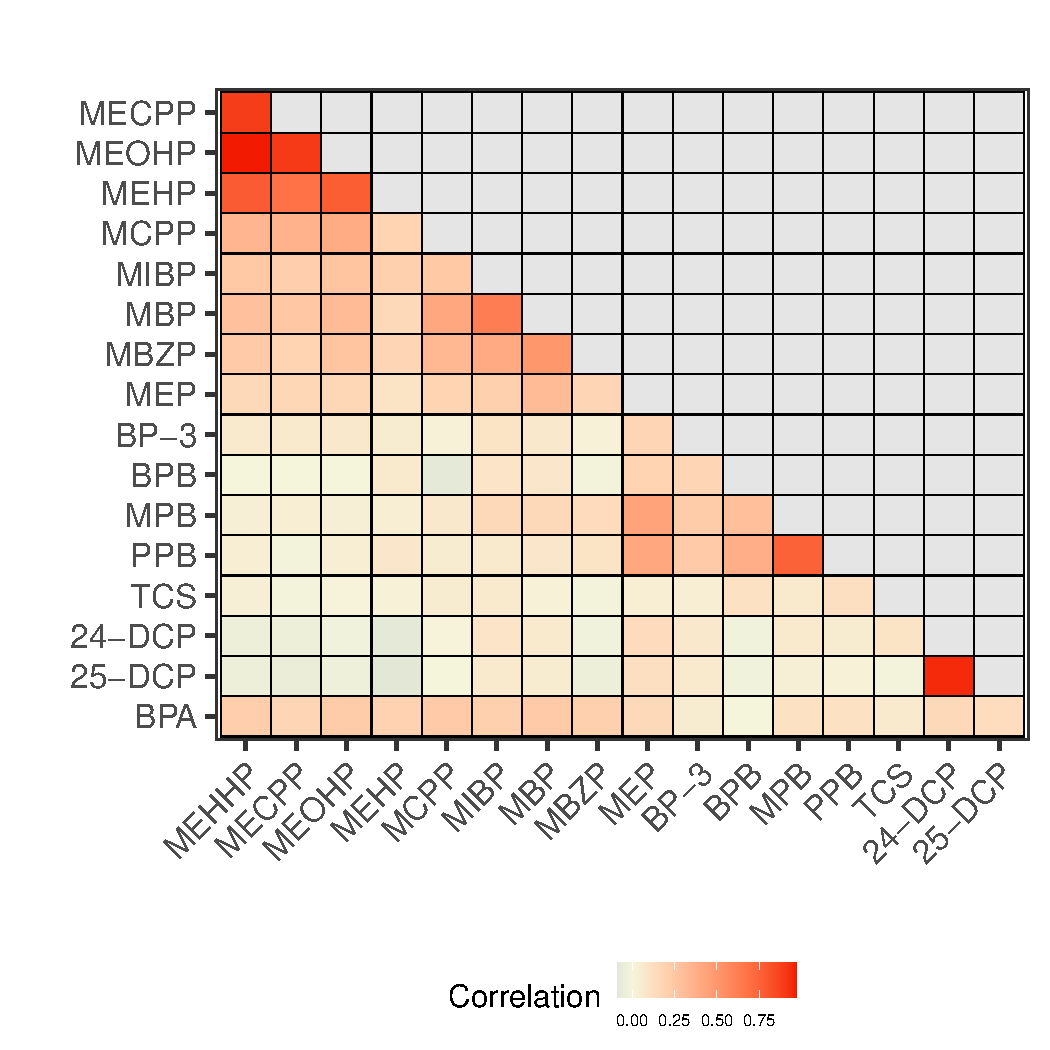
\includegraphics[scale = 0.5]{./figures/ppp_corr.pdf}
\caption{Inter-chemical correlations}
\label{fig:corr}
\end{subfigure}
\hfill
\begin{subfigure}[b]{0.3\textwidth}
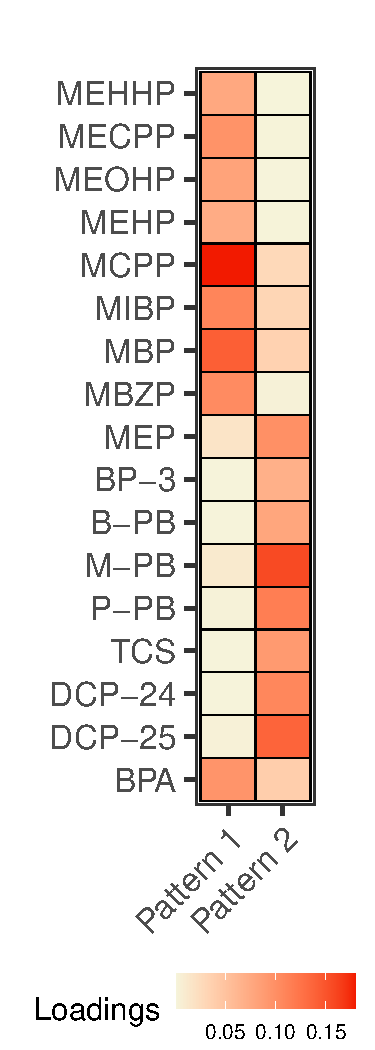
\includegraphics[scale = 0.5]{./figures/eh_loadings.pdf}
\caption{\bnmfc-identified loadings}
\label{fig:load}
\end{subfigure}
\caption[Intra-chemical correlations and \bnmfc-identified chemical loadings]{(\textbf{a}) Spearman correlations between 17 specific gravity-adjusted endocrine disrupting chemicals measured in 343 pregnant women from the Mothers \& Newborns cohort. (\textbf{b}) \bnmfc-identified chemical loadings. \bnmf discovered two underlying patterns in the mixture of seventeen phenols and phthalate metabolites in pregnant women. One pattern was characterized by phthalates and BPA, the other by phenols and MEP.}
\end{figure}

\subsection{Traditional health models}
Table~\ref{tab:reg} displays associations between prenatal exposure to \bnmfc-identified EDC patterns and child IQ in males and females from multivariable linear regression models. In these traditional regression models, we used the mean of each individual score distribution as a point estimate to assign pattern exposure. Adjusting for coviarates, full scale IQ was, on average, negatively associated with phthalate + BPA exposure in females ($\beta$ = -3.4; 95\% confidence interval (CI) = -6.5, -0.4) but not in males ($\beta$ = -0.4; 95\% CI = -2.4, 1.7). The interaction term between males and females was marginally significant (p-value $<$ 0.1). Phenols + MEP were not associated with full scale IQ in males ($\beta$ = -0.8; 95\% CI =  -2.7, 1.1), but there was suggestive evidence of a positive association in females ($\beta$ = 2.0; 95\% CI = -0.3, 4.2). The interaction term between males and females was, again, marginally significant (p-value $<$ 0.1).

\subsection{Bayesian health models}
Adjusting for covariates, full scale IQ was, on average, negatively associated with phthalate + BPA exposure in females ($\beta$ = -3.4; 95\% credible interval (CrI) = -6.7, -0.4) but not in males ($\beta$ = -0.4; 95\% CrI = -2.5, 1.7). Phenols + MEP were not associated with full scale IQ in females ($\beta$ = 2.1; 95\% CrI = -0.3, 4.5) or males ($\beta$ = -0.8; 95\% CrI = -2.8, 1.1). \\

\begingroup
\renewcommand{\arraystretch}{1.2}
\begin{table}[!h] \centering 
  \caption[Multivariable regression models of WISC-IV full scale IQ]{Results from multivariable regression models of WISC-IV full scale IQ at age seven.} 
  \label{tab:reg} 
\begin{tabular}{llrcrc} 
& & \multicolumn{2}{c}{\textit{Traditional model\textsuperscript{*}}} & \multicolumn{2}{c}{\textit{Bayesian model\textsuperscript{*}}} \\
\hline 
\\[-3ex] \hline
 & Term & $\beta$ & 95\% CI\textsuperscript{$\dagger$} & $\beta$ & 95\% CrI\textsuperscript{$\dagger$} \\ 
\hline 
\\[-3ex] \hline
\multirow{3}{*}{Phthalates + BPA} & Females          & -3.4  & (-6.5, -0.4) &  -3.4 & (-6.7, -0.4) \\ 
                           & Males            & -0.4 & (-2.4, 1.7)   &  -0.4 & (-2.5, 1.7) \\ 
                           & Interaction term & -3.1 & (-6.7, 0.6)   &  -3.0 & (-6.9, 0.6) \\ 
\hline
\multirow{3}{*}{Phenols + MEP} & Females          & 2.0   & (-0.3, 4.2) & 2.1 & (-0.3, 4.5) \\ 
                           & Males            & -0.8  & (-2.7, 1.1) & -0.8 & (-2.8, 1.1) \\ 
                           & Interaction term & 2.8   & (-0.2, 5.8) & 2.9 & (-0.1, 6.0) \\ 
\hline 
\\[-3ex] \hline \\[-2.5ex]
%\multicolumn{2}{l}{\rule{0pt}{1em}\textsuperscript{*} $p < 0.05$}\\
\multicolumn{6}{p{0.85\linewidth}}{\textsuperscript{*} Models adjusted for maternal age, IQ, and education, prenatal alcohol consumption, marital status, HOME score, and material hardship.} \\
\multicolumn{6}{p{0.85\linewidth}}{\textsuperscript{$\dagger$} 95\% CI = confidence interval for traditional regression, CrI = credible interval for Bayesian regression.} \\
\end{tabular} 
\end{table} 
\endgroup

\subsection{Sensitivity Analyses}
\subsubsection{Alternative prior distributions}
Altering the prior structure had no effect on inference. $\beta$ coefficients were, in general, unaffected or slightly farther from the null with weakly informative priors and in the hybrid scenario, and 95\% credible intervals were generally unaffected or slightly wider. As in the main analysis, full scale IQ was, on average, negatively associated with phthalates + BPA exposure in females but not in males. Phenols + MEP had no association with child intelligence. Results from Bayesian hierarchical regression models with differently-specified priors are available in Supplemental Table~\ref{tab:supreg}.

\subsubsection{Assessing effects of outlying values}
We reran multivariable regression models with the full data. We found significant deviation from linearity with the retention of these observations, which diverged from the trend in the main analysis. Supplemental Figure~\ref{fig:fulldat} contrasts our findings with the sensitivity analysis.

\section{Discussion}
% Quick recap findings
In this work, we used \bnmf to identify patterns of phenols and phthalate metabolites measured in spot urine samples from pregnant women. We saw a significant negative association between phthalates + BPA, which represented joint exposure to DEHP, di-n-butyl phthalate [DnBP], di-isobutyl phthalate [DiBP], benzylbutyl phthalate [BzBP], and BPA, and WISC-IV full scale IQ in female children at age seven. We observed no associations with phenols + MEP. We found suggestive evidence of sex-specific associations between both patterns and child IQ, though interaction terms did not reach statistical significance. Using a hierarchical Bayesian framework to incorporate the variability inherent in the pattern recognition step into the regression model, our inferences did not change. For both patterns, the direction and magnitude of the Bayesian $\beta$ coefficients matched those of the traditional models. Further, the Bayesian credible intervals, while not consistently wider, included the uncertainty of \bnmf in their coverage. This reinforces the findings of the traditional model. In quantifying the risk of cognitive deficits from EDCs---pervasive chemicals to which exposure may be preventable---we identified dietary sources of phthalates and BPA as a factor amenable to public health interventions, policy changes, or regulation.

% Continue here with summary of previous cohort results...
Our work builds on previous findings relating \textit{in utero} exposure to individual phthalates with sex-specific reductions in average child IQ in the Mothers and Newborns cohort \citep{factor2014persistent, whyatt2012maternal}. \citet{whyatt2012maternal} found negative associations between DnBP and mental development measured by the Bayley Scales of Infant Development (BSID), on average, in females at age three. \citet{factor2014persistent} extended these findings, identifying negative associations between DnBP and DiBP and average WISC-IV full scale IQ in children at age seven. DnBP and DiBP, notably, loaded strongly with phthalates + BPA in our analysis. Prenatal phthalate exposure in these children has also been linked to other developmental outcomes such as visual recognition memory \citep{ipapo2017maternal}, motor skills \citep{balalian2019prenatal, daniel2020perinatal}, and behavioral problems \citep{daniel2020prenatal}.

% Wider single chem results 
Many research groups have examined the relationship between \textit{in utero} phthalate exposure and child cognition. In another New York City cohort, \citet{engel2009prenatal} found associations between high molecular weight phthalate metabolites in pregnant women and neonatal behavior. In the same cohort, \citet{doherty2017prenatal} found lower average mental development among female children prenatally exposed to DnBP. \citet{jankowska2019phthalate} found negative associations between DnBP and dimethyl phthalate and general intellectual ability in seven year old Polish children. In a Mexican cohort, \citet{tellez2013prenatal} found a negative association between DEHP exposure and average mental development in female children between two and three years of age. In a U.S. cohort, \citet{li2019identifying} found a negative association between monobenzyl phthalate exposure at 16 weeks gestation and average full scale IQ at ages five and eight. These studies, notably, all evaluated multiple phthalates assessed individually (rather than as part of a mixture), and all reported null associations between some phthalates and child cognition \citep{radke2020phthalate}. Further inconsistency exists, as some researchers reported only null results \citep{hyland2019prenatal, nakiwala2018utero} or associations in males but not in females \citep{zhu2020domain, torres2020early, kim2011prenatal}. Variability in results may be due to a number of factors, such as timing of phthalate measurements during pregnancy, age of cognitive assessment in the children, cognitive tests measuring different constructs (e.g., WISC-IV vs. BSID), insufficient adjustment for confounders (potentially including other phthalate metabolites), varying phthalate concentrations in study populations, or differences in the distributions of distinct effect modifiers in the study population. 

\bnmf also identified a second pattern representing phenols and MEP that was not associated with child IQ. However, previous 
research has shown association between individual phenols and child cognition. In a U.S. cohort, \citet{jackson2018identifying} found maternal urinary triclosan concentrations at delivery were associated with lower cognitive test scores, on average, in eight year old children of both sexes. \citet{freire2020association} found placental concentrations of PPB were associated with poorer memory and motor function, on average, in Spanish children between four and five years of age.

% other mixtures results
Because individuals are not exposed to phenols or phthalates in isolation, research increasingly aims to account for simultaneous exposures to these chemicals as environmental mixtures. Within this area of research, different statistical methods have been employed to answer different questions \citep{gibson2019complex}. For example, weighted quantile sum (WQS) regression has been used to answer research questions concerning the overall effect of an EDC mixture on child cognition and the identification of potential chemicals of concern \citet{tanner2020early, loftus2021exposure}.

Beginning with a research question more similar to our own, \citet{kalloo2021chemical} used k-means clustering, a traditional pattern recognition tool, to identify pregnant women with similar chemical exposure profiles within a mixture of EDCs (including phenols and phthalates), metals, and environmental tobacco smoke. In a two-stage analysis, they found that children born to women in the k-means-identified `cluster 1' had lower scores on the performance IQ subscale compared with the reference cluster. Membership in `cluster 1' indicated higher concentrations of DEHP metabolites, MBP, BPA, triclosan, and BP-3, among others, and lower exposure to parabens, MBZP, MIBP, and MEP. While our results are not directly comparable, both studies identified relationships between patterns or profiles expressing exposure to DEHP metabolites and BPA and child IQ, though \citet{kalloo2021chemical} found no evidence of sex-specific associations.

% what's cool about \bnmf
We originally adapted \bnmf to environmental epidemiology to address specific impediments to pattern recognition in environmental mixtures. First, we cannot know the true underlying number of patterns. To reduce the need for \textit{post hoc} pattern selection and foster reproducibility of analyses, \bnmf includes an empirical sparse prior to choose the number of patterns in the mixture. Second, epidemiologists and environmental heath scientists generally desire interpretable patterns, as opposed to solely dimension reduction. \bnmfc's non-negative priors return results on an additive scale that encourages interpretability \citep{lee1999learning}. Finally, as in this analysis, pattern recognition in environmental health is often followed by a health model to estimate relationships between patterns and outcomes. Traditional methods ignore any uncertainty in pattern identification. \bnmf provides score distributions that can propagate uncertainty into health models.

% limitations
Our findings should be interpreted in light of several limitations. First, as is the case when using chemical biomarkers, our study is susceptible to exposure measurement error, which may have biased our estimates towards the null. Second, some components may be metabolized faster than others, and our mixture includes measurements from both parent compounds and metabolites. If components with shorter half-lives are more toxic and their levels are not adequately captured in the single sample provided by the participants, this could impact both the \bnmf solution and the subsequent health effect estimates. Repeat measurements have shown that these markers fail to reliably approximate continuous exposure \citep{fisher2015bisphenol, braun2012variability}. However, previous research in the Mothers and Newborns cohort showed moderate to high intra-class correlation coefficients, indicating consistency over time \citep{whyatt2012maternal, factor2014persistent}. Third, our findings may not be generalizable to a more general population; our cohort is composed of low-income Dominican and African American mothers living in an urban environment, and the \bnmfc-identified EDC patterns may represent sources or behaviors distinct to this group. Fourth, Bayesian models, in general, are powerful in their ability to combine information from multiple sources (i.e., data and prior information), but when initial assumptions are wrong, the conclusions will be as well. We evaluated our models with posterior predictive checks and used both noninformative and weakly informative priors in an ongoing process of feedback and quality control. Fifth, our dataset is high-dimensional, with a large number of correlated chemical measurements for each participant. In this situation, \bnmf performs exceptionally, as it was first designed for geothermal spectrograms, sensor measurements of frequencies over time, which are at a finer resolution and higher dimension than our current problem domain \citep{holtzman2018machine}. Finally, though we adjusted for multiple factors that varied across households to account for potential confounding, we cannot exclude the possibility of residual confounding.

Our study has a number of strengths. First, the prospective cohort design ensures the temporal ordering of exposure and outcome. Second, all phenols and phthalate metabolites were measured at the CDC; their quality assurance/quality control reduces the possibility of bias in measurement. Third, the WISC-IV test has measured reliability and validity and is sensitive to effects of low-dose neurotoxicant exposures on cognition \citep{rauh2011seven, jusko2008blood, wechsler2003wechsler}. Finally, our statistical methods appropriately address our research question concerning the relationship between patterns of prenatal EDC exposure and child cognition. \bnmf incorporates joint exposures in identified patterns, which better reflects the entire EDC milieu than individual measurements. Our two-stage hierarchical Bayesian health model propagates the uncertainty from \bnmf in the subsequent regression model, providing robust results and improving inference.

\section{Conclusion}

Our analysis identified two patterns of phenol and phthalate exposure in pregnant women. One pattern grouped metabolites of several phthalates and BPA, which are commonly found in food containers and packaging; the other grouped the remaining phenols, including parabens and triclosan, with the metabolite of DEP, all of which are more prevalent in personal care products. We detected a significant association between phthalates + BPA and average full scale IQ in females, but not males, at age seven. These results add to a body of evidence that, though somewhat 
inconsistent, indicates harmful and often sex-specific effects of EDCs in child development. By measuring prenatal patterns of EDCs, we identified an exposure source resembling food packaging as a potential risk factor most amenable to policy changes or regulation.

\clearpage
\setcounter{figure}{0}
\setcounter{table}{0}
\renewcommand{\thefigure}{S\arabic{figure}}
\renewcommand{\thetable}{S\arabic{table}}
\section{Supplemental Materials}

\subsection{Alternative prior distributions}
\label{sec:priors}
Noninformative prior specifications on the Bayesian model made the resulting parameter estimates more comparable with our traditional model. In Bayesian statistics, however, `weakly' informative priors are generally preferred because noninformative priors place a large portion of their probability mass on unreasonable parameters. In our example with child IQ as the outcome, a noninformative prior on $\beta$ implies that we believe a coefficient of $\pm$ 100 is as likely as a coefficient of zero, which is, of course, implausible. Weakly informative priors, on the other hand, contain enough information to regularize the posterior distribution (i.e., to keep it between relatively reasonable bounds), but they do not attempt to fully capture previous beliefs or to heavily weight scientific knowledge about underlying parameters \citep{bda3}. We set up two scenarios, one with weakly informative priors and the other with a combination of weakly informative and noninformative priors, as sensitivity analyses. These encoded information about parameters and we designed them so as not to overly influence the posterior. Our weakly informative priors were modeled after \citet{gelman2020regression}. We fit two alterative prior structures, (1) weakly informative, where the $\beta$ distribution for phthalates + BPA was based on previous results (explained below) and all other coefficients were centered at zero, and (2) weakly informative/noninformative hybrid, where the $\beta$ distribution for phthalates + BPA was based on previous results, the $\beta$ for phenols + MEP was distributed around zero, and all covariates kept noninformative priors. The two schemes included the same priors on $\alpha$, $\sigma$, and the $\beta$ coefficients of interest as follows,
\begin{equation*}
\begin{aligned}
& \alpha \sim \mathcal{N}(100, 45), 
& \sigma \sim \operatorname{Exponential}(\frac{1}{sd_y}), \\
& \beta_{PHT+BPA} \sim \mathcal{N}(-1.19, 2.5 \cdot sd_y), 
& \beta_{PHT+BPA \cdot s} \sim \mathcal{N}(-0.03, 2.5 \cdot sd_y), \\
& \beta_{PHN+MEP} \sim \mathcal{N}(0, 2.5 \cdot sd_y), 
& \beta_{PHN+MEP \cdot s} \sim \mathcal{N}(0, 2.5 \cdot sd_y)
\end{aligned}
\end{equation*}

Here, $sd_y$ is the standard deviation of the observed full scale IQ. $\beta_{PHT+BPA}$ and $\beta_{PHN+MEP}$ are the coefficients for the phthalate + BPA pattern and the phenol + MEP pattern, respectively; $\beta_{PHT+BPA \cdot s}$ and $\beta_{PHN+MEP \cdot s}$ are the coefficients for the corresponding interaction terms with sex. The weakly informative and weakly/non- informative hybrid structures differed only in the prior distributions on covariates. In the first scenario, $\beta_{\ldots} \sim \mathcal{N}(0, 2.5 \cdot sd_y)$ to serve as a soft regularizers, where $\beta_{\cdots}$ includes the coefficients for sex and all covariates. In the second, priors on sex and other covariates were flat over $\beta_{\ldots} \sim \mathcal{U}(-\infty, \infty)$, so as not to affect inference. Because WISC-IV IQ scales are standardized to a mean of 100 and a standard deviation of 15 \citep{wechsler2003wechsler}, we modeled $\alpha$ as normally distributed around 100 with a wider standard deviation. The specified distributions and parameters for $\sigma$ and the $\beta$ coefficients also considered the scale of the outcome \citep{gelman2020regression}. The error in the model was drawn from an exponential distribution with rate $= \frac{1}{sd_y}$; this placed the bulk of the distribution below $sd_y$, with a long right tail to accommodate uncertainty. Weakly informative priors on $\beta$ coefficients for patterns and interaction terms were normally distributed. For phthalates + BPA, we used \citeauthor{factor2014persistent}'s results to determine our prior means. They estimated sex-specific individual associations between full scale IQ and five of the eight phthalate metabolites that loaded strongly with phthalates + BPA \citep{factor2014persistent}. We took the average coefficient size across the five reported in that paper in males as phthalates + BPA's prior mean. We took the average difference between coefficients in females and males as the prior mean of the interaction between phthalates + BPA and sex. We had no prior knowledge on the association between phenols + MEP and full scale IQ, so for phenols + MEP and the pattern's interaction term with and sex, we set the means to zero. For both patterns and both interaction terms, we set the standard deviation to $2.5 \cdot sd_y$ to make these priors only weakly informative. 

\clearpage
\begin{landscape}
\begingroup
\renewcommand{\arraystretch}{1.075}
\begin{table} \centering 
%\small
  \caption[Subject demographics in parent cohort and study population]{Subject demographics and distribution of potential confounders, model covariates, and outcome variable in full Mothers and Newborns cohort (N = 727), subsample with phenols and phthalates measured in urine (N = 343), subsample with full scale WISC IQ measured at age 7 (N = 311), and subsamples with no missing covariates (N = 289).} 
  \label{tab:suptable1} 
\begin{tabular}{l|rr|rrr|rrr|rrr}
\hline
\hline
\multirow{2}{*}{Characteristic} & \multicolumn{2}{c}{Entire Cohort} & \multicolumn{3}{c}{\bnmf Subsample} & \multicolumn{3}{c}{WISC Subsample} & \multicolumn{3}{c}{Complete Cases} \\
& \multicolumn{2}{c}{N = 727} & \multicolumn{3}{c}{N = 343} & \multicolumn{3}{c}{N = 311} & \multicolumn{3}{c}{N = 289} \\
\hline
 & \multicolumn{2}{c}{Value\textsuperscript{*}} & \multicolumn{2}{c}{Value\textsuperscript{*}} & P\textsuperscript{$\dagger$} & \multicolumn{2}{c}{Value\textsuperscript{*}} & P\textsuperscript{$\dagger$} & \multicolumn{2}{c}{Value\textsuperscript{*}} & P\textsuperscript{$\dagger$} \\
\hline
Ethnicity & & & & & $>$0.9 & & & 0.9 & & & $>$0.9 \\
\hspace{1em}African American & 254 & 34.9 & 119 & 34.7 & & 107 & 34.4 & & 100 & 34.6 & \\
\hspace{1em}Hispanic/Latina & 473 & 65.1 & 224 & 65.3 && 204 & 65.6 && 189 & 65.4 & \\
\hline
Maternal education & & & & & 0.8 & & & 0.8 & & & $>$0.9 \\
\hspace{1em}$\le$ High school degree or equivalent & 456 & 64.0 & 216 & 63.0 && 196 & 63.0 && 186 & 64.4 & \\
\hspace{1em}$<$ High school degree                 & 257 & 36.0 & 127 & 37.0 && 115 & 37.0 && 103 & 35.6 & \\
\hline
Material hardship & 321 & 44.2 & 144 & 42.0 & 0.5 & 128 & 41.2 & 0.4 & 116 & 40.1 & 0.2 \\
\hline
Marital status & & & & & 0.5 & & & 0.6 & & & 0.5 \\
\hspace{1em}Never Married & 473 & 65.4 & 232 & 67.6 && 209 & 67.2 && 195 & 67.5 & \\
\hspace{1em}Ever Married & 250 & 34.6 & 111 & 32.4 && 102 & 32.8 && 94 & 32.5 & \\
\hline
Prenatal alcohol consumption & 192 & 26.4 & 91 & 26.5 & $>$0.9 & 77 & 24.8 & 0.6 & 72 & 24.9 & 0.6 \\
\hline
Smoker in home & 246 & 33.8 & 103 & 30.0 & 0.2 & 94 & 30.2 & 0.3 & 89 & 30.8 & 0.4 \\
\hline
Child sex & & & & & 0.6 & & & 0.6 & & & 0.6 \\
\hspace{1em}Male & 376 & 51.7 & 184 & 53.6 && 166 & 53.4 && 155 & 53.6 & \\
\hspace{1em}Female & 351 & 48.3 & 159 & 46.4 && 145 & 46.6 && 134 & 46.4 & \\
\hline
Maternal age at delivery & 25.2 & 4.9 & 25.6 & 4.9 & 0.2 & 25.5 & 4.9 & 0.2 & 25.6 & 4.9 & 0.2\\
\hline
Maternal IQ & 85.5 & 13.3 & 85.2 & 13.6 & 0.5 & 84.9 & 13.4 & 0.4 & 84.8 & 13.5 & 0.3 \\
\hline
HOME scale & 39.4 & 6.3 & 39.5 & 6.3 & $>$ 0.9 & 39.3 & 6.3 & 0.7 & 39.4 & 6.2 & 0.9\\
\hline
Child Full Scale IQ & 98.5 & 12.9 & 97.3 & 13.3 & 0.2 & 97.3 & 13.3 & 0.2 & 97.3 & 13.4 & 0.2\\
\hline
\multicolumn{12}{l}{\rule{0pt}{1em}\textsuperscript{*} Value = n, \% or Mean, SD}\\
\multicolumn{12}{p{21cm}}{\rule{0pt}{1em}\textsuperscript{$\dagger$} P = p-value from Pearson's Chi-squared test for categorical variables; Wilcoxon rank sum test for continuous variables. Tests of the difference in distributions between the entire cohort and the three nested subsamples.} \\
\end{tabular}
\end{table}
\endgroup
\end{landscape}

\clearpage
\begingroup
\renewcommand{\arraystretch}{1.2}
\begin{table} \centering 
  \caption[Bayesian hierarchical models of WISC-IV full scale IQ]{Results from Bayesian hierarchical regression models of WISC-IV full scale IQ at age seven with alternative prior specifications.} 
  \label{tab:supreg} 
\begin{tabular}{llrcrc} 
& & \multicolumn{2}{c}{\textit{Weakly informative\textsuperscript{1}}} & \multicolumn{2}{c}{\textit{Weakly/non-informative\textsuperscript{1}}} \\
\hline 
\\[-3ex] \hline
 & Term & $\beta$ & 95\% CrI\textsuperscript{2} & $\beta$ & 95\% CrI\textsuperscript{2} \\ 
\hline 
\\[-3ex] \hline
\multirow{3}{*}{Phthalates + BPA} & Females          & -3.5 & (-6.6, -0.4) & -3.4 & (-6.6, -0.4) \\ 
                           & Males            & -0.4 & (-2.5, 1.7)  & -0.4 & (-2.5, 1.6) \\ 
                           & Interaction term & -3.1 & (-6.8, 0.6)  & -3.0 & (-6.8, 0.7) \\ 
\hline
\multirow{3}{*}{Phenols + MEP} & Females          & 2.1  & (-0.2, 4.5) & 2.1 & (-0.2, 4.5) \\ 
                           & Males            & -0.8 & (-2.8, 1.2) & -0.8 & (-2.8, 1.1) \\ 
                           & Interaction term & 2.9  & (-0.1, 6.0) & 2.9 & (-0.1, 6.0) \\ 
\hline 
\\[-3ex] \hline \\[-2.5ex]
%\multicolumn{2}{l}{\rule{0pt}{1em}\textsuperscript{*} $p < 0.05$}\\
\multicolumn{6}{p{0.9\linewidth}}{\textsuperscript{1} Models adjusted for maternal age, IQ, and education, prenatal alcohol consumption, marital status, HOME score, and material hardship.} \\
\multicolumn{6}{p{0.75\linewidth}}{\textsuperscript{2} 95\% CrI = credible interval.} \\
\end{tabular} 
\end{table} 
\endgroup

 \clearpage
\begin{figure}
\centering
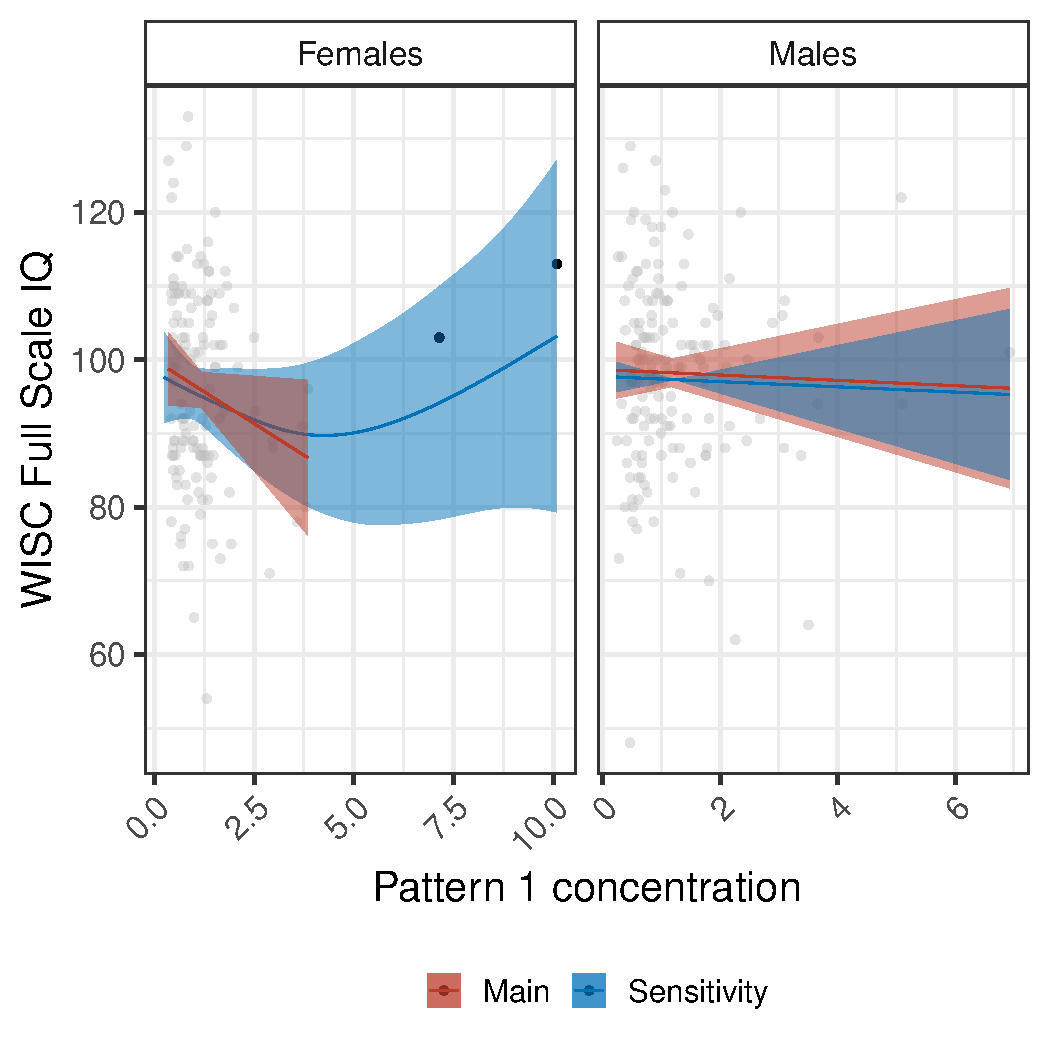
\includegraphics[scale = 0.85]{./figures/sense_plot.pdf}
\caption[Sensitivity analysis of associations in main analysis and full study sample]{Associations between phthalate + BPA pattern concentrations in pregnant women and children's full scale IQ at age 7 in the main analysis and sensitivity analysis. Models adjusted for maternal age, IQ, and education, prenatal alcohol consumption, marital status, HOME score, and material hardship. Shaded areas include 95\% confidence bands. Points represent measured data, with two influential outliers colored in black. Retaining these values in the data caused a deviation from linearity in females. Both extreme observations belonged to female children; their exclusion did not affect the relationship in males.}
\label{fig:fulldat}
\end{figure}

\clearpage
